

\clearpage
\section{Realisierung}\label{sec:Realisierung}

Das digitale Theremin ist auf dem Entwicklungsboard DE1-SoC von Terasic aufgebaut. Dieses enthält ein Cyclone V 5CSEMA5 FPGA von Intel. Weiter befindet sich auf dem Board der Audio Codec WM8731 von Wolfson für die Ausgabe an einem Lautsprecher. In Abbildung \ref{img:Blockschaltbild_top} ist der Aufbau des digitalen Theremin aufgezeigt inklusive der Peripherie ausserhalb des FPGA.\\
Das Theremin, welches im FPGA aufgebaut ist, besteht aus zwei Bereichen. Einerseits der Signalverarbeitung und Übermittlung an den Codec. Dieser besteht aus den Komponenten \textit{Lautstärke}- und \textit{Tonhöhenverarbeitung}, \textit{DC-FIFO} und dem \textit{Audioserialisierer}. Der zweite Bereich ist Das Nios II System. Dieses besteht aus dem Prozessor und diversen IP Cores, welche die Kommunikation mit den Peripherien ermöglicht. Ausserhalb des FPGA ist zudem das entwickelte PCB, welches die beiden Antennenoszillatoren enthält und das Spielen des Theremin ermöglichen.\\
Die Kommunikation zwischen dem Nios II Prozessor und den anderen Komponenten geschieht über das \textit{Avalon Memory Mapped Interface}. Der Prozessor ist in dieser Kommunikation Master und die restlichen Komponenten Slaves. Die Übertragung der Audioinformation in der Signalverarbeitung geschieht über das \textit{Avalon Streaming Interface}. Wobei Sender als Streaming Source und Empfänger als Streaming Sink deklariert sind. Das Streaming Interface ist notwendig für den Einsatz des Dual-Clock-FIFO (DC-FIFO). Dieses übernimmt den Übergang verschiedener Clockregionen zwischen den Komponenten \textit{Tonhöhenverarbeitung} und \textit{Audioserialisierer}.\\
Die Clocks, welche zu den verschiedenen Komponenten gehen sind in Abbildung \ref{img:Blockschaltbild_top} für eine bessere Übersichtlichkeit weggelassen worden. Für eine Liste aller Clock Frequenzen und deren Ziel siehe Kapitel \ref{subsec:Clock}.

\begin{figure}[h!]
	\centering
	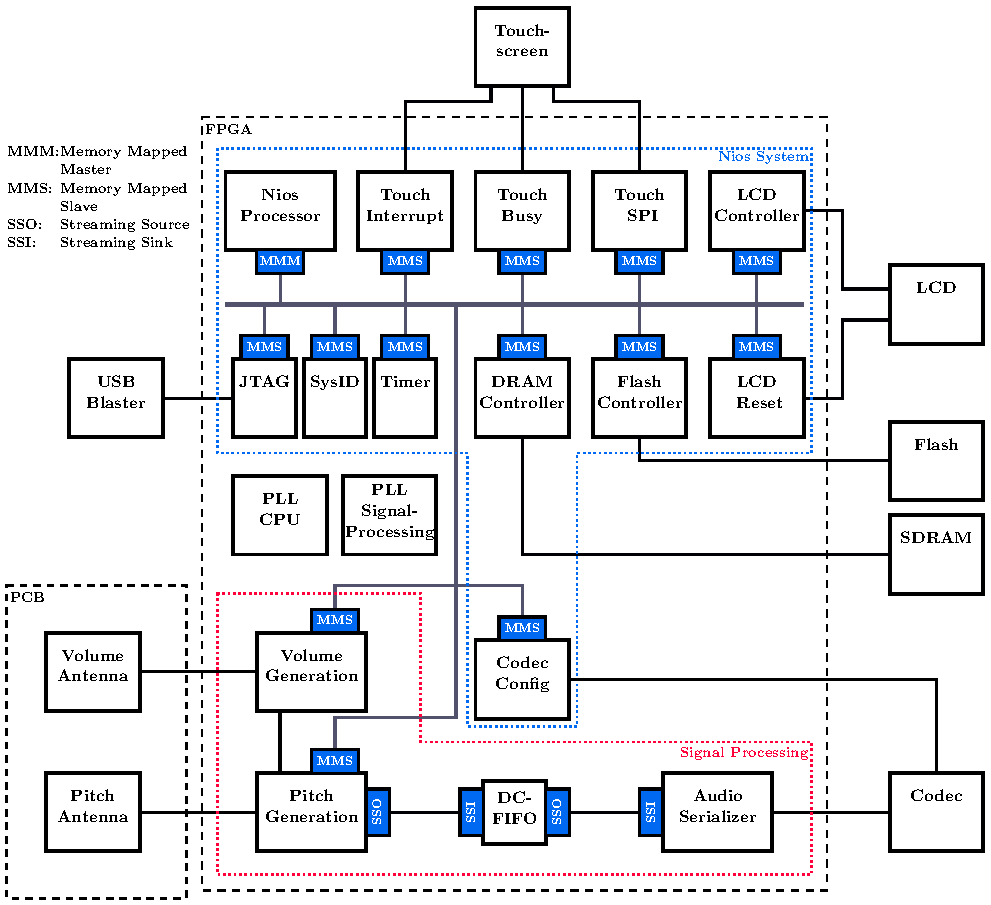
\includegraphics[width=1\textwidth]{Blockschaltbild_top.pdf}
	\caption{Blockschaltbild gesammtes Theremin} 
	\label{img:Blockschaltbild_top}
\end{figure}  

\clearpage

